\chapter{Design and Implementation}
\label{chapter:design}

Based on the requirements identified in the previous chapter, we're in this chapter introducing the design and implementation details of the of our proposed proxy solution. We get started by discussing the overall design, before we dive into the implementations details.



\section{Design of Solution}

In previous chapters we have argued that all optimization techniques should be
placed in proxies in order to retain interoperability for COTS applications, as
well as to break the end-to-end dependency. Our design therefore involves deploying a
proxy pair to facilitate Web communication. The idea is to deploy the proxy pair
in two different locations separated by a DIL network. Through the locally
deployed proxy, Web applications can proxy all their data communication. The
proxy will then apply different optimization techniques and over a DIL
network forward the request to the other proxy, and finally return a response.
Ideally should a proxy be deployed as close to its intended user applications as
possible, preferable at the same machine.


It is worth noting that since the proxies is designed to accept \textit{all} HTTP
requests, they can support any applications that utilize HTTP, including request-
response and publish-subscribe applications.


\subsection{Design of HTTP proxy}

A deployed proxy is designed to accept arbitrary HTTP requests, possible originating from
multiple clients, and forward them to the other proxy as seen in
\cref{figure:proxy_design}. Ideally the proxy should be deployed as close to its
intended users as possible, as the communication between an application and its
proxy is not subject to any optimization for DIL environments.

\begin{figure}[h]
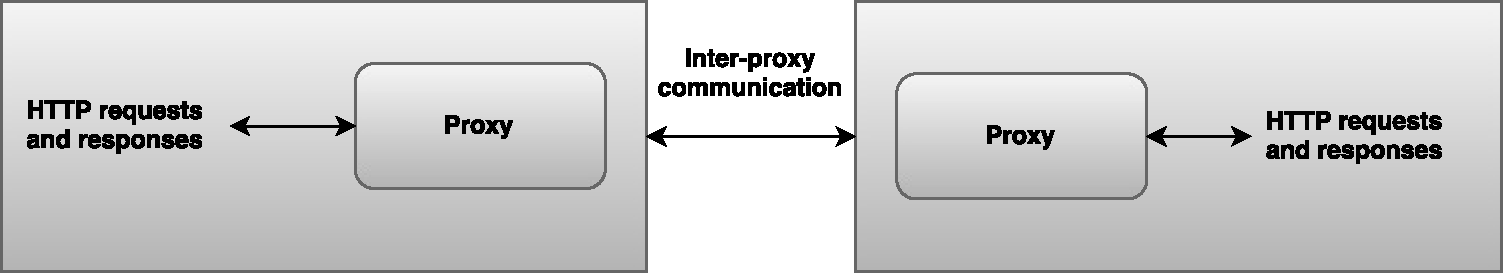
\includegraphics[scale=0.55]{images/proxy_design.pdf}
\caption{Design of Solution}
\label{figure:proxy_design}
\end{figure}

It is the communication between a proxy pair that is subject to optimizations.
The proxies are therefore designed to support the optimization techniques we
have identified. Those are primarily concerned about using different transport
protocols as the inter-proxy communication, as illustrated in
\cref{figure:proxy-communication}. The purpose of this is to evaluate the
performance of the transport protocols in DIL networks. Which protocol to use as
the means of inter-proxy communication is therefore designed to be easily
configured by the user of the proxy.

\begin{figure}[h]
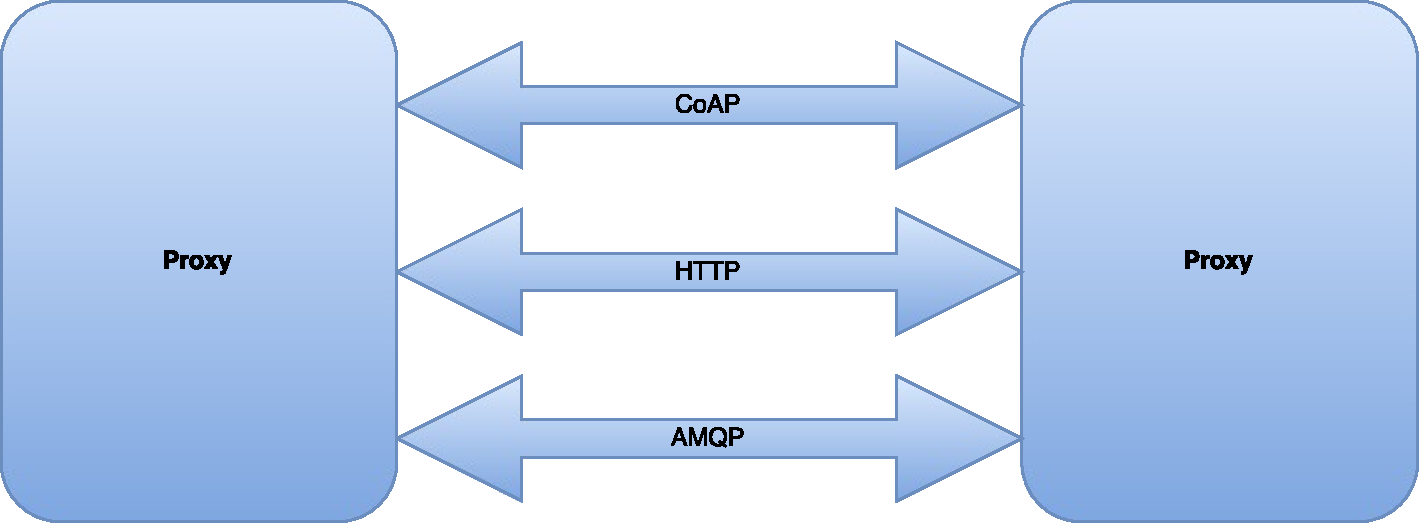
\includegraphics[scale=0.5]{images/proxy_communcation.pdf}
\caption{The proxies were designed to support multiple protocols for inter-proxy communication}
\label{figure:proxy-communication}
\end{figure}

\subsection{Message Broker}

ActiveMQ 5-13.2

\section{Choosing a Framework}

Requirement one implies creating a HTTP proxy which accepts HTTP requests,
forward them, and finally return a HTTP response. We identified some approaches:

\begin{enumerate}
    \item Build a HTTP proxy from scratch ourselves.
    \item Use an existing HTTP proxy.
\end{enumerate}

Building a HTTP proxy ourselves would allow us to customize our solutions as we
wanted, but would require a lot of implementation. We therefore concluded that
best use of our resources was to use an existing configurable proxy.
Building on existing solutions allows us to focus on the optimization techniques,
rather than on the specific low-level details of HTTP.
There are numerous HTTP proxies available for use, for an example Nginx and Squid.

Another one is Apache Camel, which is an open source Java framework developed by
the Apache Software Foundation for rule-based routing and
mediation \cite{camel-homepage}. It has a wide range of use-cases and focuses on
making integration between different enterprise communication systems easier. It
support a large set of different communication transports (transport protocols).
We chose to use Apache Camel as our HTTP proxy due to its simplicity and support
for different transport protocols.

\subsection{Apache Camel}

Routing is a central concept in Apache Camel and consists of defining a
\textit{from route}. This is an endpoint from which Camel consumes messages. It
can then invoke a series of \textit{processors}, which can modify the headers,
payload etc. of the message. Then, Camel forwards the message to a \textit{to
route}, which can be an application running somewhere else. When a response is
received, Camel can invoke a new set of processors on the message, before it is
finally returned to the origin. An overview of this can be seen in
\cref{figure:camel-route}.

\begin{figure}[h]
\centering
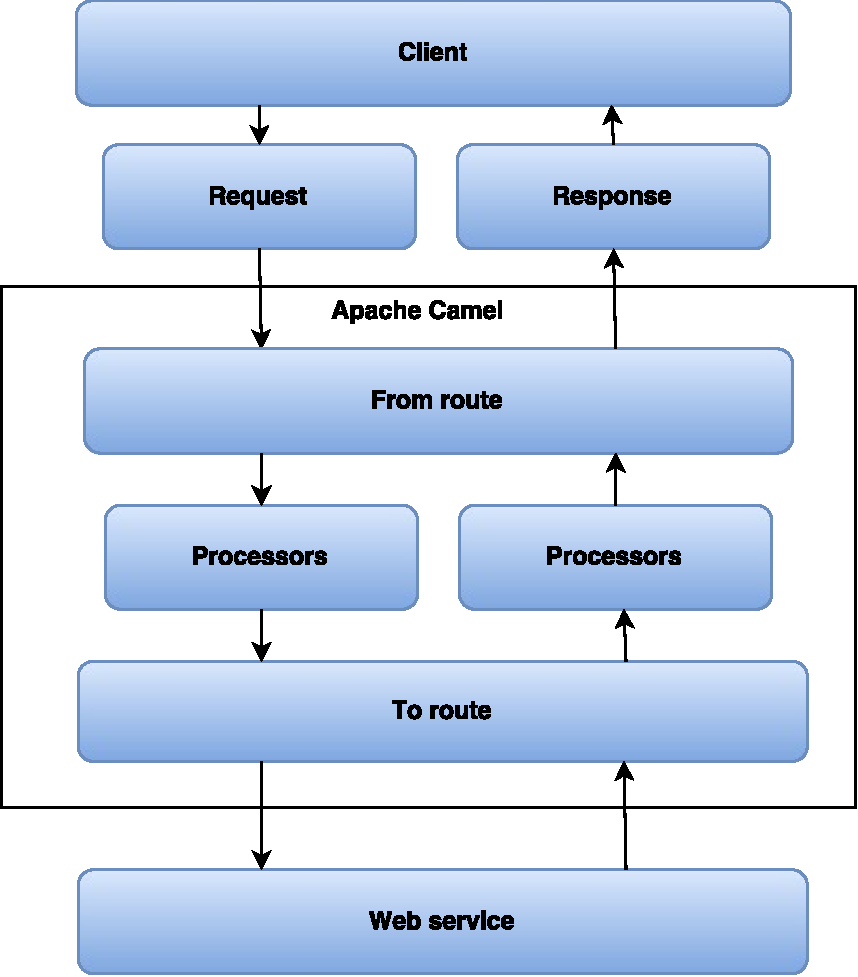
\includegraphics[scale=0.7]{images/camel_routes.pdf}
\caption{Example of a Camel route}
\label{figure:camel-route}
\end{figure}

To consume and produce messages from different protocols, databases and other
sources of messages, Camel offers a set of \textit{components}. These
can be considered as factories for endpoint instances. For example, the AMQP
component allows Camel to route messages using the AMQP protocol. Camel includes
numerous components, and is designed to support user written components as well.


\section{Implementation}

The proxy is implemented as a Java 1.8 application using the Apache Camel
framework. A large part of the implementation is concerned about reading user
configuration and setting up \textit{routing rules} for Apache camel. The stages
of the program are as follows:

\begin{enumerate}
    \item Reading and parsing user configuration.
    \item Initializing Camel components.
    \item Setting up routes.
    \item Running.
\end{enumerate}

\subsection{Parsing Configuration}

The first stage involves reading a user provided configuration file. Details
about the configuration is explained in \cref{section:proxy-config}.

\subsection{Initializing Components}

Depending on which protocol the user has selected for usage as inter-proxy
communication, at startup the respective Camel component is initiated and added
to the Camel context. Due to the time available, we did not implement support for all of the
recommended protocols from the last chapter. The currently supported protocols
are HTTP, AMQP and CoAP. However, the proxy is designed to by easily extendable to
include additional protocols.

\subsubsection{HTTP Component}

We made use of the Camel component Jetty in order to consume and produce HTTP
requests. The component is based on the Jetty Web server\cite{jetty-homepage}
and is used for two purposes. One of them is to consume \gls{http} requests from
 applications. The other is to, if HTTP was configured as the selected protocol,
 to consume and produce HTTP messages as part of the inter-proxy communication.

\subsubsection{AMQP Component}

Apache Camels AMQP component supports the AMQP 1.0 protocol using the JMS Client
API of the Qpid project. JMS is a Java Message Oriented Middleware for sending
messages between two or more clients. In the proxy component initialization
phase, the AMQP component is initialized to connect to the configured broker. In
addition, the request timeout value of an AMQP request is set either to the
default value of 20 seconds, or to the configured value.

\subsubsection{CoAP Component}

At the time of writing this thesis, there was no Camel component available for
the CoAP protocol. We therefore implemented our own custom component, supporting
the transport of CoAP messages. The component utilizes Californium, which is a
Java framework supporting the CoAP protocol \cite{californium-homepage}.
Californium is open source and is part of the \gls{iot} ecosystem of Eclipse.
The component is initialized with the port the CoAP server should listen for
requests. In addition, an optional timeout value for a CoAP request can be added.

\subsection{Routes}

A running proxy listens on two \textit{routes}. It can either receive messages
from an application, or it can receive a message from the other proxy. This
setup can be seen in \cref{figure:dil-routes}. The routing logic is different
for these two cases. We define a request originating from an outside application
as the \textit{application route}, and a request originating from another proxy
as the \textit{proxy route}. We discuss these routes shortly, but first we need to
introduce what we have chosen to call the \textit{proxy message format}.
Requirement 2 says that we need to retain all the original HTTP headers from the
original request. Consider if the proxy receives a HTTP request and forwards it
to the other protocol using AMQP. The message itself will arrive correctly, but
the original HTTP headers and method would be lost. Our approach to this was to
introduce a custom \textit{proxy message format}, which is discussed in
\cref{section:proxy-header-format}.

\begin{figure}[h]
\centering
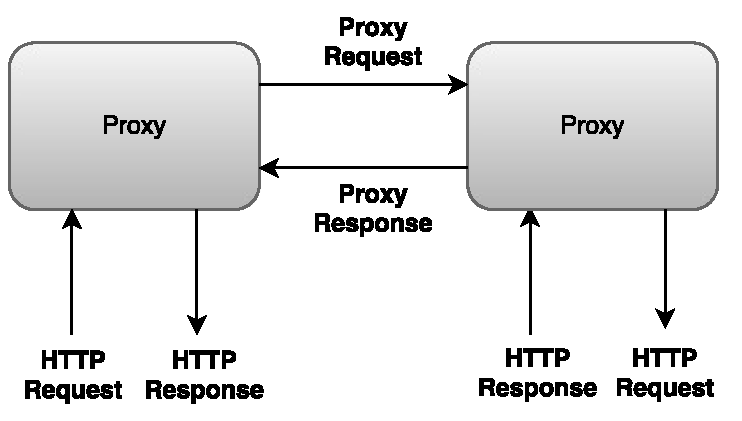
\includegraphics[scale=0.7]{images/dil_routes.pdf}
\caption{Proxy routes}
\label{figure:dil-routes}
\end{figure}



\subsection{Proxy Message Format}
\label{section:proxy-header-format}

The proxy message format was developed to retain HTTP headers and other
necessary information about the request. Our solution was to wrap all messages
in a \gls{json} document and include necessary information as properties in the
JSON document. JSON is a lightweight, text-based data format \cite{rfc-json}. We
chose this data format due to its compactness, simplicity and the wide support
for libraries for generating and parsing JSON. Due to a HTTP request and
response having slightly different semantics, we used the same format, but
with different properties for a request and response. The request format is
defined in \cref{table-proxy-request}, and the response format in
\cref{table-proxy-response}.

\begin{table}[h]
\begin{tabularx}{\textwidth}{|l|X|l|}
\hline
\textbf{Field} & \textbf{Purpose}                                                                                                      & \textbf{Required} \\ \hline
path           & The original request URL from the application. Specifies the intended final destination of the original HTTP request. & Yes               \\ \hline
method         & HTTP method of the request.                                                                                           & Yes               \\ \hline
query          & Query string associated with the original HTTP request.                                                               & No                \\ \hline
headers        & JSON object containing all the original HTTP headers of the request                                                   & Yes               \\ \hline
body           & The original payload of the message                                                                                   & No                \\ \hline
\end{tabularx}
\caption{Proxy message request fields}
\label{table-proxy-request}
\end{table}

\begin{table}[h]
\begin{tabularx}{\textwidth}{|l|X|l|}
\hline
\textbf{Field} & \textbf{Purpose}   & \textbf{Required} \\ \hline
headers        & JSON object containing the HTTP response headers. & Yes  \\ \hline
responsecode   & The HTTP response code. & Yes \\ \hline
body           & Response body of the HTTP request. & No            \\ \hline
\end{tabularx}
\caption{Proxy message response fields}
\label{table-proxy-response}

\end{table}

An example proxy request message is included in \cref{listing:proxy-request}.
The listing illustrates a HTTP request originating from an outside application.
It is a HTTP POST to the intended destination http://myservice.com, with a XML
message as payload.

\lstinputlisting[frame=single, language=json, firstnumber=1, caption="Example proxy request", label=listing:proxy-request]{listings/proxy_message.json}

\paragraph{}

\subsection{Application Route}

The purpose of the application route is to consume HTTP requests from an outside
HTTP request, transform it to a proxy request message and deliver it to the
other proxy using the configured protocol. The semantics of the protocol
specific routes are explained in \cref{section:protocol-routes}. When a response
from the other proxy is received, it is returned to the application which made
the request. The route consists of the following steps:

\begin{enumerate}
	\item Defining a HTTP endpoint to consume HTTP requests from. This is read from the configuration which specifies which hostname and port to listen on.
	\item Consume HTTP request from an outside application
	\item Apply the \textit{ProxyRequestPreProcessor}. This processor converts the message into a Proxy Request Message.
	\item If compression is enabled, compress the entire message.
	\item Forward the request to the other proxy using the configured transport protocol.
	\item Receive a response from the other proxy.
	\item If compression is enabled, de-compress the message.
	\item Restore the HTTP response from Proxy Response Message.
	\item Return the response to the application.
\end{enumerate}

\subsection{Proxy Route}

The purpose of the proxy route is to listen for messages from the other proxy,
de-serialize it, and deliver it to its intended receiver. When a response is
received, transform it into a Proxy Response Message and return it to the other
proxy. The route consists of the following steps:

\begin{enumerate}
	\item Defining an endpoint depending on which the configured protocol.
	\item Consume requests from the other proxy.
	\item If compression is enabled, de-compress the message.
	\item Transform the message into the original HTTP request.
	\item Forward the HTTP request to its intended destination.
	\item Receive a HTTP response from the intended destination.
	\item Transform it into a Proxy Response Message.
	\item If compression is enabled, compress the message.
	\item Return the response to the other application.
\end{enumerate}

\subsection{Protocol Specific Routes}
\label{section:protocol-routes}

Depending on which protocol the user has configured for inter-proxy
communication, the endpoint defining the interface between the proxies is
defined. \Cref{table:example-endpoints} lists example endpoints of a deployed
proxy. In the example the other proxy is located at the IP address
192.168.10.10. We discuss the protocol specific semantics in the following
paragraphs.

\begin{table}[h]
\begin{tabular}{|l|l|l|}
\hline
\textbf{Component} & \textbf{Consume endpoint} & \textbf{Produce endpoint}       \\ \hline
HTTP               & http://0.0.0.0:3001/proxy & http://192.168.10.10:4001/proxy \\ \hline
AMQP               & amqp:queue:uniquename1    & amqp:queue:uniquename2          \\ \hline
CoAP               & coap://0.0.0.0:3001/proxy & coap://192.168.10.10:4001/proxy \\ \hline
\end{tabular}
\caption{Example endpoints for a deployed proxy.}
\label{table:example-endpoints}
\end{table}


\subsubsection{HTTP Route}

If HTTP is configured as the inter-proxy communication protocol, two HTTP
endpoints are defined. The first is used to consume from, while the second is
used to produce to. From the user provided configuration the \textit{hostname}
and \textit{port} is retrieved, and the proxy starts listening on this endpoint.
Note that the HTTP component is also used to listen on requests from other
applications. Therefore only requests with an \gls{uri} starting with a
\textit{proxy} prefix will be treated as an incoming proxy message.

In the same way, the produce endpoint is defined. The target hostname of the
other proxy is retrieved from the configuration and the \textit{proxy} prefix
is appended.

\subsubsection{AMQP Route}

AMQP messaging is based on the concept of queues. For the routing of messages
 between the proxies, we define two queues.
 One queue for incoming messages to one of the proxy,
 and one queue for incoming messages to the other proxy.
 A proxy then consumes messages from its incoming messages queue
 and produces to the queue for incoming messages of the other.

\subsubsection{CoAP Route}

The CoAP route is similar to the HTTP route. It listens on the provided hostname
and port, and produces messages to the configured hostname of the other proxy.


\subsection{Dealing with Errors}

If an error occurs during the routing of a message, for example a timeout
exception, the default Camel error handling is to propagate the error back to
the requester. One of our requirements is that the proxy should be able to deal
with disconnects. We therefore need to handle exceptions that occur during
routing in a more elegant way. Note that this applies to the routing between the
proxies, the \textit{proxy route}.

We implement this by using the \textit{DeadLetterChannel} error handler rather
than the default error handler. The DeadLetterChannel allows us to configure the
redelivery policy according to the configuration of the proxy. This can either
be with an exponential delay or with a fixed delay. Finally, the maximum number
of redelivery attempts is set. This number can be set to infinity.

\subsection{Runtime}

In the running stage, the proxy listens on the defined routes and forwards
 requests according to the previously configured routes. All requests passing
 through the proxy are logged to the console.


\section{Functionality}

The proxy prototype is packaged as a JAR file and can be started from the command
line as seen in \cref{listing:proxy-start}. The path to a valid configuration
file must be passed as a command line argument.

\lstinputlisting[frame=single, language=json, caption="How to start the proxy", label=listing:proxy-start]{listings/proxy_start.sh}

\subsection{Configuration of Proxy}
\label{section:proxy-config}

The configuration of a proxy is done by passing configuration files as argument
to the proxy at startup. In the configuration, the user can specify settings
such as which protocol to use for inter-proxy communication and compression
settings. We use the typesafe\cite{typesafe-homepage} configuration library to
parse configuration files. The supported configuration options of the proxy are
listed in \cref{appendix-config} in the appendix.

\Cref{listing:proxy-config} lists an example configuration of a proxy. The proxy
is configured to listen on port 3001 for messages from applications and forward
them using the AMQP protocol. Messages sent to the other proxy are configured to
be sent uncompressed. At initialization the proxy connects to the broker at the
given location. It will consume messages on the given \textit{consumeQueue} and
produce messages to the \textit{produceQueue}.


\lstinputlisting[frame=single, language=json, firstnumber=1, caption="Example proxy configuration file", label=listing:proxy-config]{listings/amqp.conf}


\subsection{Proxy Setup}

In order to enable the applications to tunnel all their HTTP traffic through our
proxy, we need a way to set a proxy without altering the applications
themselves. Fortunately, Java provide mechanisms to deal with proxies
\cite{oracle-proxy}. We configured the \gls{jvm} to get the applications to
tunnel all HTTP traffic through our proxy. This is done by setting properties to
the \gls{jvm}:


\begin{lstlisting}[frame=single, language=json, caption="Setting a proxy on the \gls{jvm}", label=test]
java -Dhttp.proxyHost=localhost \
-Dhttp.proxyPort=3001 \
-Dhttp.nonProxyHosts= \
-jar target/client.jar
\end{lstlisting}

In \cref{test} the application \textbf{client.jar} is started and all HTTP
traffic will go through the proxy server at localhost on port 3001.


\section{Software Used}

The proxy is implemented in Java using the Apache Camel framework.
\Cref{table:implementation-versions} lists the software versions used in the
implementation.

\begin{table}[h]
\begin{tabular}{|l|l|}
    \hline
\textbf{Software} & \textbf{Version} \\ \hline
Java            & 1.8           \\ \hline
Apache Camel     & 2.16.1           \\ \hline
camel-amqp      & 2.16.1            \\ \hline
camel-jetty      & 2.16.1            \\ \hline
javax.jms-api      & 2.0            \\ \hline
Californium      & 1.0.0            \\ \hline
typesafe      & 1.3.0            \\ \hline
\end{tabular}
\caption{Software used in the proxy implementation}
\label{table:implementation-versions}
\end{table}

\section{Summary}

In this chapter we presented the design and implementation details of the proxy.
